%!TEX root = thesis.tex
\chapter{Method}
\label{chapter:Method}

Empirical research by its very nature relies heavily on quantitative information and a means of analysing this information. In our study, we extract information from number of \OSYS. This chapter introduces the different types of information that can be used to study software evolution, the Open Source Software Systems that were used for our analysis and the approach to selecting systems. Following this, we outline how we defined vocabulary and the method we used to extract vocabularies from the selected systems.

\section{Data Collection} % (fold)
\label{sec:data_collection}

% - Need to first identify an appropriate source of information for study evolution

% - Need to source individual systems that maintain a complete record of their history

% - Refine according to some criteria

\subsection{Types of Evolution Data} % (fold)
\label{sub:types_of_evolution_data}

% - We used the release history as it presents concrete outcomes, whereas the revision history relies too much on human factors.

Studies of software evolution rely on historical information relating to software systems. Using this information, we can construct a longitudinal representation of the software in order to analyse its evolution. This historical information falls under three classifications, as described in \cite{Vasa10a}, which are summarised in Table~\ref{tab:Histories}.

\begin{table*}[t]
\centering
\begin{tabular}{|p{.23\textwidth}|p{.72\textwidth}|}
\hline
{\bf History} & {\bf Description}\\
\hline \hline
Release History & Source code, binaries, release notes, and release documentation\\
\hline
Revision History & Version control logs, issue/defect records, Modification history of documentation, Wiki logs\\
\hline
Project History & Messages (email, Instant message logs), Project documentation (plans, methodology, process)\\
\hline
\end{tabular}
\vspace{0.2cm}
\caption{The different types of histories that typically provide input data for studies into software evolution}
\label{tab:Histories}
\vspace{-0.2cm}
\end{table*}

\emph{Release history} is that which is composed of data that pertains to the releases of a software system. This is most commonly source code, but can also include binaries, release notes and release documentation. Studies of the release history of software systems focus upon the outcome of changes within a software system. \emph{Revision history} on the other hand, relates to the information captured regarding change, composed of information such as version control logs, defect logs and other change documentation. Such information allows us to understand the maintenance activities of the developers involved and how it relates to change. \emph{Project history} is information relating the communication and process of those involved with the project, including email and IM logs, as well as project documentation capturing plans, methodology and process.

% - Reword paragraph below

For our study we directly analysed the release history of the software systems; more specifically, the binaries that represented individual releases. This allowed us to study the product of development efforts and gave us something concrete to study; it was also the most consistenly available information. As both \emph{revision history} and \emph{project history} rely too much on human factors, this information was used as an insight in the development practices of the software and helped guide our investigation.

% subsection types_of_evolution_data (end)

\subsection{Open Source Software (OSS)} % (fold)
\label{sub:open_source_software_oss_}

% \crumbs{\textbf{Why do we use OSS?}}
% 
% \crumbs{\textbf{OSS is, in general, software that is free. -- Raj}}
% 
% \crumbs{\textbf{It has non-restrictive licensing, which allows us to use and modify it as we see fit.}}
% 
% \crumbs{\textbf{It is popularly used, even within commercial projects}}
% 
% \crumbs{\textbf{It is this liberal approach to licensing that makes OSS an attractive option for }}

% - OSS is free and distributed with source code

% - Gained adoption within commercial projects

% - Generally have liberal licensing schemes which allows developers to do what they want with the code

% - Allows us an insight into the practices of developers that would not be available in commercial projects due to protection of information

% - Distributed...people from many backgrounds

% - Availability of not only current state of software, but also an entire history (source code, documentation, change logs)

% subsection open_source_software_oss_ (end)

\subsection{Obtaining the Data} % (fold)
\label{sub:obtaining_the_data}

% - Glue sentence -- we need a lot of data!

To obtain the raw data required for conducting our study, we drew upon an existing corpora of open source Java software systems known as the Helix data set \cite{Helix10a}, which was established and used as a component of the work undertaken by Vasa in \cite{Vasa10a}.

The Helix data set was composed by mining many popularly used open source project repositories. Such repositories provide a rich source of information pertaining to the studies of software. This typically includes the source code and binary packages for most, if not all, of the versions that have been released as part of the project. In addition to this, most repositories provide tools such as source control, wikis and defect tracking that facilitate communication between the developers of the project and the user base.

\bigskip
The data set was composed of projects obtained from the following repositories:
\begin{enumerate}
	\item Sourceforge - {\em http://www.sourceforge.com}
	\item OW2 Consortium - {\em http://www.objectweb.org}
	\item Apache Software Foundation - {\em http://www.apache.org}
	\item Java Community Projects - {\em http://community.java.net/projects/}
	\item Google Code - {\em http://code.google.com}
	\item Eclipse Project - {\em http://www.eclipse.org}
	\item Netbeans Project - {\em http://www.netbeans.org}
\end{enumerate}

Furthermore, we refined the Helix data set which was presented in \cite{Vasa10a} to include an up to date release history for each of the systems within the data set.

% subsection obtaining_the_data (end)

\subsection{Selection Criteria} % (fold)
\label{sub:selection_criteria}

In order to identify suitable systems for our study, we defined a number of selection criteria. The set of criteria used and the rationale for our selection is presented in this section.

In order to selecting suitable systems for our study, we leveraged a selection criteria used for studying \OSYS in the context of software evolution, as proposed by Vasa in \cite{Vasa10a}.

In their study they define the following criteria that each project considered for selection must meet:

\begin{enumerate}
	\item The system must be developed for the Java virtual machine. Source code and compiled binaries are available for each release.
	\item The software is a single coherent system, that is, it is a distribution of a collection of related {\em components} packaged together.
	\item At least {\em 15 releases} of the system are available. Only complete releases with a version identifier are considered. Branches and releases not derived from the main system tree are ignored.  Minor and major versions are both considered (for instance, Version 2.0, 2.1 and 3.0 are all considered. In this case, the version with identifier 2.1 is often a release that provides minor enhancements and/or defect corrections).
	\item The system has been in actively development and use for at least \emph{36 months}.
	\item The system comprises of at least \emph{100 types} (i.e., classes and interfaces) in all releases under study.
	\item Change logs do exist. This data provides the additional information to understand the rationale behind the changes.
\end{enumerate}

\subsubsection{Rationale of Selection Criteria} % (fold)
\label{ssub:rationale_of_selection_criteria}

In \cite{Vasa10a} the rationale that was provided can be summarised as:

% - Java is popular and is widely used

% - Subsequently, lots of software has been developed using it

% - 36 months chosen as an indicator of projects that are likely to be mature in their development. Took a subset of projects that were considered to be successful. More likely have a significant development history.

% - Systems that at least 100 class were chosen as they were less likely to trivial and we would be able to generalise on bigger systems.

% - Changes logs would help to guide our investigation and explain anomalies and big changes.

% They noted that size and skill of development teams was removed as criteria as this information could not be accurately established.

% subsubsection rationale_of_selection_criteria (end)

% subsection selection_criteria (end)

\subsection{Selected Systems} % (fold)
\label{sub:selected_systems}

% Glue sentence -- we had more systems to choose from, but we didn't for X reasons

The subset of the systems that were selected from the Helix data set to use for our study consists of \emph{thirty-four} systems which, altogether, account for 1011 unique releases and approximately 34,000 classes (between each of the systems and their releases).

These systems were selected with the intention of achieving a near-equal representation of a diverse range of different types of software available in the Java open source community. Broadly, they fall within one of three categories: (a) Applications, (b) Frameworks, and (c) Libraries, as defined in \cite{Vasa10a}.

\emph{Applications} are software systems that are able to be executed in isolation and provide functionality that is independent of other software systems. Meanwhile, \emph{Frameworks} and \emph{Libraries} are systems that provide functionality that is designed to be extended or re-used by other software systems through an API defined by the developers. Frameworks differ from libraries in that they intend to provide an abstraction that is to be extended by those using it in order to make use of it in their systems, whereas libraries typically encapsulate functionality that is used directly within the application. As there is a fine line between whether a piece of software is considered a \emph{Framework} or a \emph{Library}, the classification was derived from the terminology used by the development team responsible for a given project. A summary of the systems that were selected and how they were categorised is provided in Table~\ref{tab:systems}.

%%% Components/Frameworks that were analyzed %%%
\begin{table*}[!]
\centering
\small
\vspace{-0.6cm}
\begin{tabular}{|l|l||c|c|r|p{0.38\textwidth}|}
\hline
{\bf Name} & {\bf Type} & {\bf Rel.} & {\bf Age} &
             {\bf Size} & {\bf Description}
\\
\hline \hline
Ant&Application&18 & 510 & 561 & Build Management System\\
\hline
Azureus&Application&52 & 348 & 3261 & Bittorrent Client\\
\hline
Checkstyle&Application&19 & 365 & 270 & Static Code Quality Checker\\
\hline
DataVision&Application&18 & 325 & 233 & Reporting tool\\
\hline
Findbugs&Application&20 & 282 & 1044 & Defect identification tool\\
\hline
Flow4J&Application&29 & 94 & 274 & Process flow modeling\\
\hline
Groovy&Application&42 & 345 & 965 & Scripting language\\
\hline
JChempaint&Application&23 & 346 & 986 & Chemistry Visualisation\\
\hline
JMeter&Application&21 & 418 & 692 & Testing tool kit\\
\hline
JabRef&Application&32 & 327 & 868 & Bibliography management\\
\hline
Jasperreports&Application&63 & 426 & 1439 & Reporting engine\\
\hline
Kolmafia&Application&102 & 265 & 662 & Role Playing Game\\
\hline
Maven&Application&15 & 225 & 437 & Build management system\\
\hline
PMD&Application&42 & 345 & 570 & Static code checker\\
\hline
Proguard&Application&24 & 417 & 561 & Java Obfuscator\\
\hline
SoapUI&Application&26 & 246 & 1400 & SOAP header monitoring tool\\
\hline
\hline
Cocoon&Framework&15 & 420 & 692 & Web application framework\\
\hline
Hibernate&Framework&60 & 438 & 1893 & Object Relational Mapping\\
\hline
Jena&Framework&25 & 452 & 915 & Semantic Web Framework\\
\hline
Spring&Framework&55 & 363 & 2593 & Lightweight J2EE framework\\
\hline
Struts&Framework&18 & 469 & 910 & Web Application Framework\\
\hline
Velocity&Framework&24 & 475 & 229 & Templating engine\\
\hline
Webwork&Framework&21 & 218 & 505 & Web App. Development\\
\hline
Wicket&Framework&39 & 295 & 803 & Web App. Development\\
\hline
XWork&Framework&26 & 288 & 304 & Generic Command Pattern\\
\hline
Freemarker&Library&17 & 390 & 287 & Template engine\\
\hline
JFreeChart&Library&21 & 377 & 587 & Charting library\\
\hline
Jung&Library&25 & 324 & 358 & Universal Graph Library\\
\hline
Log4J&Library&17 & 421 & 215 & Logging framework\\
\hline
Lucene&Library&19 & 418 & 398 & Text search engine\\
\hline
Quartz&Library&17 & 376 & 177 & Job Scheduling System\\
\hline
Saxon&Library&31 & 375 & 937 & XML and XSLT processor\\
\hline
Xalan&Library&15 & 400 & 1198 & XSLT Processor\\
\hline
Xerces&Library&20 & 496 & 710 & XML processor\\
\hline
\end{tabular}
\caption{Systems investigated - Rel. shows the total number of distinct releases analyzed. Age is shown in Weeks since the first release. Size is a measure of the number of classes in the last version under analysis.}
\label{tab:systems}
%\vspace{-0.2cm}
\end{table*}

% subsection selected_systems (end)

% section data_collection (end)

\section{Vocabulary Extraction} % (fold)
\label{sec:vocabulary_extraction}

% - To capture representation of vocabulary that can be analysed, need to first identify which elements are considered parts of the vocabulary and which are not (dissemination)

% - Once this has been identified need a way of extracting this information and presenting it in a way in which it can be analysed.

% - In this section we describe how this achieved...

\subsection{Vocabulary Definition} % (fold)
\label{ssec:vocabulary_definition}

% Introduce section

% What should consitute a definition of vocabulary, based upon what is usually considered vocabulary (definition)

\subsubsection{Existing Definitions of Vocabulary} % (fold)
\label{ssub:existing_definitions_of_vocabulary}

Research in the area of source code vocabulary is currently lacking an adequate and consistent definition of vocabulary.

% This was highlighted by Delorey et al. in \cite{Delorey09a}.


In their study, they outlined a number of possible definitions of what constitutes a \emph{word} within source code, the atomic unit with which vocabularies are composed.

% Their study defined \emph{word} at the syntactic level of abstraction.

% - Group lexicographically equivalent words only if they are used as the same part of speech

% - For example, a class name and a function name that are lexicographically isomorphic are counted as separate words

% - By using syntactic knowledge intelligently, they are are able to differentiate the definition of a word from its use. This allows us to detect polysemy and make approximate adjustments in our analyses

% - This also included mathematical operators

% subsubsection existing_definitions_of_vocabulary (end)

\subsubsection{Defining Vocabulary} % (fold)
\label{ssub:defining_vocabulary}

% Glue sentence -- Development is usually carried out by teams ... the usage of vocabulary is less likely to influence an individual as they form their own mental model with the code, whereas when mutliple developers are involved there is more of a need for this information to be shared and communicated accordingly.

Accordingly, our definition of vocabulary has an emphasis on the elements of source code that are likely to be experienced by multiple developers, as opposed to an individual.

% Flow:
% - We ignore language that is used in a localised scope (more speficially this means we ignore things into to methods...)

% - We focus on the language utilised by the developers for a project. It should be something that reflects the decision process of the developers involved in the project. Thus, we ignore elements of the vocabulary that developers do not have a choice in (refer to eliminating noise section)

% - Section~\ref{ssub:eliminate_noise_in_the_vocabulary}

% - Language that is used within a non-localised scope. Vocabulary defined within methods is self-contained. Therefore it usually not seen or dealt with by a lot of developers (can something be cited here?).

% - Our definition prefers to deal with abstraction that are likely to be present to developers both involved in the development of the software and those who might programmatically use the software, but who are external to its development.

% - We considered the set of class names, method names and field names to be apart of the vocabulary within source code of a software system.

% subsubsection defining_vocabulary (end)

% subsection vocabulary_definition (end)

\subsection{How the Data is Extracted} % (fold)
\label{sub:how_the_data_is_extracted}

For extracting the representation of vocabulary we used for our analysis from each of the software systems within our dataset, we utilised the \emph{Mutations} software evolution metric extraction analysis tool, which was described in \cite{Vasa10a}. Mutations utilises the ASM bytecode analysis and manipulation framework to extract metadata associated with a Java class from its compiled binary state (.class).

Amongst the metadata collected by the tool is information relating to the members of the class (i.e. its methods and fields). This information includes, for fields, the name of the field and its type; for methods, the name of the method, its return type and the types of each of its parameters. This metadata provided the elements from which we composed the vocabulary.

In order to extract the terminology that composed the vocabulary, we extended Mutations to support the extrapolation of individual terms from these elements.

\subsubsection{Identifying Terms in the Source Code} % (fold)
\label{ssub:identifying_terms_in_the_source_code}

Best practices relating to naming identifiers within source code recommend using names that clearly and effectively communicate the purpose of what they represent. The result of this is that developers quite often utilise identifiers that are composed of multiple words. However, for the purposes of our study we considered each word that an identifier is composed of as a separate term within the vocabulary. For example, the identifier \emph{MainWindow} would be separated into two individual terms, \emph{main} and \emph{window}. 

In order to separate compound identifiers into the individual terms that they are composed of, we required appropriate guidelines to assist us in determining when an identifier has been composed of more than one term. For our purposes, we utilised the Java Coding Style Guide \cite{Reddy00a}, which is well adhered to within the open source community, as it has style guides for developers which apply alternative casing and delimiter characters to allow easier identification of individual terms within an identifier.

For the naming of identifiers at any level of abstraction, the Java Coding Style Guide prescribes the following naming styles:

\begin{description}
	\item[Pascal case] Each word begins with an uppercase letter, followed by all lowercase letters\\ (e.g. ReportWriter produces \textbf{report} and \textbf{writer})
	\item[Camel case] First word begins with a lower case letter, followed by all lowercase letters. Each trailing word beings with an uppercase letter, followed by all lowercase letters\\ (e.g. writeReport produces \textbf{write} and \textbf{report})
	\item[Upper-case and underscore separated] Each word is composed of all capital letters and words are separated by an underscore\\ (e.g. MAX\_REPORT\_LENGTH produces \textbf{max}, \textbf{report} and \textbf{length})
\end{description}

The application of these naming conventions as it relates to the elements that make up our vocabulary are defined as follows:

\begin{description}
	\item[Class names] Pascal case
	\item[Method names] Camel case 
	\item[Field names] Camel case (instance variables), upper-case and underscore separated (constants)
\end{description}

% subsubsection identifying_terms_in_the_source_code (end)

\subsubsection{Eliminate Noise in the Vocabulary} % (fold)
\label{ssub:eliminate_noise_in_the_vocabulary}

% Perhaps need a glue sentence here: Developers use shared vocabulary across projects...get/set/int/string/,  are common conventions used by programmers, particularly in the Java community [Cite Java coding style guide]. While this kind of information is useful in communicate intent to those may read the code, these kinds of terms are well understood by developers and are unlikely to lead to any cognitive disruption...

% - May unreasonably cause noise in detecting big changes in vocabulary

To allow for a representation of vocabulary that reflected the choice of terminology utilised by the developers involved with a given project, we elected to discount terms that were overwhelmingly the most commonly used across all of the projects we analysed.

Our initial observations showed that the most frequently used terms across all of the projects we selected consisted primarily of the primitive types available within the Java language. As developers are bound by the language itself to use the types, they did not fall within our definition of vocabulary. Additionally, the frequency of their usage was sufficiently high that they were likely to deter the ability to detect changes in the rest of the vocabulary.

Amongst the most frequently used terms, were those prescribed by the naming conventions to be used for writing Java code outlined in \cite{Reddy00a}. This included terms such as \emph{get} and \emph{set}, terms used for naming acessors and mutators within Java programs. As conformance to such coding styles is mandated by most successful \OSYS, these terms were also ignored.

We were able to refine our subset of vocabulary further by identifying terms that were ambiguous and not contributing any substantial meaning to the vocabulary, but were commonly found terms within each of the projects. For instance, the terms \emph{data}, \emph{name} and \emph{value} are all terms that are typically used in conjunction with other terms and on their own have very low semantic value.

Taking the notion of isolating vocabulary that was more likely to be project-specific a step further, we also compiled a list of the data structure and I/O types available within the Java SDK to be excluded from our analysis. This included extensions of primitive types (e.g. BigDecimal, BigInteger), collection types (e.g. ArrayList, HashMap), as well as types used for accessing data streams (e.g. InputStream, OutputStream).

A complete list of both the terms that were excluded from the representation of vocabulary that we analysed can be found in Chapter~\ref{cha:cha:vocabulary_analysis_files}.

% subsubsection eliminate_noise_in_the_vocabulary (end)

% subsection how_the_data_is_extracted (end)

\subsection{Extraction Algorithm} % (fold)
\label{sub:extraction_algorithm}

In order to extract the vocabulary from the metadata collected by Mutations, we added a module within the tool to take the relevant data that had been extracted as a result of processing each of the versions for a given system and extract the terms from each of the elements identified in the previous section.

The process begins by first extracting the information required to build the vocabulary from individual classes for a given release. For each class in the version being processed, we take the name of the class, as well as its set of methods and fields and extract the information required to build the vocabulary. This step consists of taking each of the elements of the different abstractions we highlighted in the previous section and isolating the identifiers within these elements. Utilising the naming conventions presented in the previous section, we separate the identifiers into individual terms. For each level of abstraction, we maintain the number of times a term has occurred.

Once the individual terms have been extracted from each of these elements, we take the term occurrence counts that were stored for class names, methods and fields and combined them into one representation of the number of times a term has been used in a class, representing the vocabulary usage for the class. While doing this, we also filter out any of the terms that were considered to be noise, as described in the previous section. Sample code highlighting the elements that are extracted from the code to represent the vocabulary for the class is shown in Listing~\ref{lst:extraction_example}. In the sample listing, the terms \emph{report}, \emph{settings}, \emph{break}, \emph{print} and \emph{writer} have been extracted and form the vocabulary for the class, while the terms \emph{get}, \emph{set} and \emph{string} have been eliminated as noise terms.

Finally, we take the vocabulary we extracted for each class and combine them together to form the vocabulary for the version as a whole, as represented by a collection of all the terms used and the number of times which they were used in the version.

\begin{figure}[t]
\centering
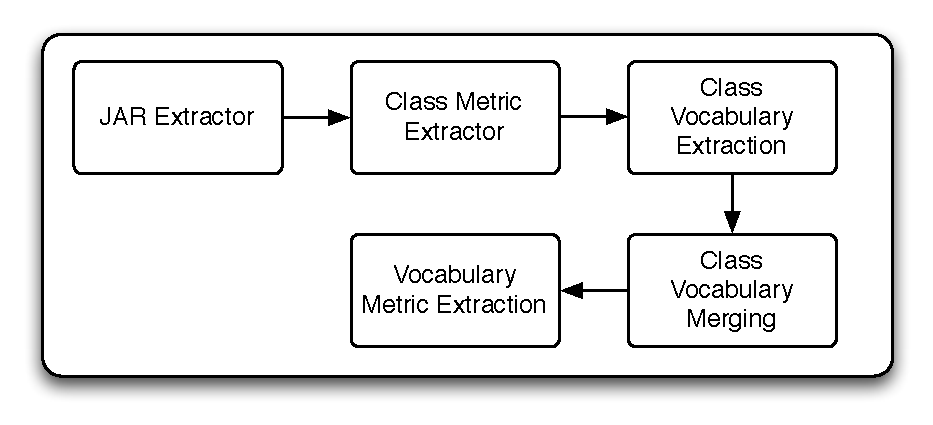
\includegraphics[width=\textwidth]{Figures/Vocab-VocabMetricExtraction.pdf}
\caption{Vocabulary metric extraction process for each release of a software system}
\label{fig:vocab-metric-extraction}
\end{figure}

\begin{lstlisting}[caption={Code sample showing the extraction of terms from various elements of the source code}, label={lst:extraction_example}, float=t]
public class ReportWriter // report, writer (class name)
{   
    // string (type); report, break (name)
    private static final String REPORT_BREAK = "----------";

    // report, settings (type); settings (name)
    private ReportSettings settings;
    
    // report, settings (return type); get, report, settings (name)
    public ReportSettings getReportSettings()
    {
        return settings;
    }
    
    // set, report, settings (name); report, settings (parameter type)
    public setReportSettings(ReportSettings settings)
    {
        this.settings = settings;
    }
    
    // print, report (name); report (parameter type)
    public void printReport(Report report)
    {
        System.out.println(REPORT_BREAK);
        
        if(settings.isTitleOutputted())
            System.out.println(report.getTitle());
            
        System.out.println(report.getBody());
        System.out.println(REPORT_BREAK);
    }

	/** Term occurrences: **/
	// - report: 9
	// - settings: 5
	// - break: 1
	// - print: 1
	// - writer: 1
	// - get: 1  (noise term -- ignored)
	// - set: 1  (noise term -- ignored)
	// - string: 1  (noise term -- ignored)
}
\end{lstlisting}

% // Class Name: ReportWriter
% // report, writer
% 
% // Constant field: String REPORT_BREAK
% // - string, report, break
% 
% // Instance variable: ReportSettings settings
% // - report, settings; settings
% 
% // Method: getReportSettings()
% // - get, report, settings (return type); report, settings (method name)
% 
% // Method: setReportSettings(ReportSettings settings)
% // - set, report, settings (method name); report, settings (method parameter type)
% 
% // Method: printReport(Report report)
% // - print, report (method name); report (method parameter type)
% 
% // Term occurrences:
% // - report: 9
% // - settings: 5
% // - break: 1
% // - print: 1
% // - writer: 1
% 
% // Noise terms eliminated:
% // - get
% // - set
% // - string

% subsection extraction_algorithm (end)

% section vocabulary_extraction (end)

\section{Summary} % (fold)
\label{sec:summary}

% Summarise what was covered...

% - What types of evolution data were outlined
% - We study OSS
% - Vocabulary is defined as ...

% In the next chapter we address the research questions proposed in regard to the evolution of vocabulary. We...



% section summary (end)